%!TeX root = main.tex
\chapter{Beispiel}

\section{Allgemein} \label{sec:allgemeinProblem}

\begin{comment}
siehe: \cite[5.b]{sabbah_Fourier-local}
\end{comment}

\begin{comment}
sei $\phi\in\{\frac{1}{t^k},\frac{1}{t^2}+\frac{1}{t^3},\dots\}$
\begin{enumerate}
\item Starte mit: $P(t,\partial_t):=(\partial_t-\frac{d}{dt}\phi(t)) \cdot
\mbox{Hauptnenner }\in\C[t]<\partial_t>$
\item Furiertrafo: $F_P(z,\partial_z)=P(\partial_z,-z)\in\C[z]<\partial_z>$
\item $x=z^{-1}$ und $\partial_x=-z^2\partial_z$ \\
\[
Q(x,\partial_x):=F_P(x^{-1},-x^2\partial_x)\cdot \mbox{Hauptnenner
}\in\C[x]<\partial_x>
\]
\item Berechne für $Q$ das NP usw...
\end{enumerate}
\end{comment}

Hier wollen wir nun eine Spezielle Klasse von Meromorphen Zusammenhängen, die
die durch das folgende Rezept entstehen.
\begin{enumerate}
\item Wähle ein $\phi$ zB. aus
$\{\frac{1}{t^k},\frac{1}{t^2}+\frac{1}{t^3},\dots\}$
\item und beginne dann mit
\[
\tilde P(t,\partial_t):=(\partial_t-\frac{d}{dt}\phi(t))
\]
\item Multipliziere mit Hauptnenner
\[
P(t,\partial_t):=(\partial_t-\frac{d}{dt}\phi(t)) \cdot
\mbox{Hauptnenner }\in\C[t]<\partial_t>
\]
\item wende auf $P$ die Fouriertransformation 
$F_P(z,\partial_z)=P(\partial_z,-z)$ an und erhalte ein Element
in $\C[z]<\partial_z>$
\item Wende die Übergänge $x=z^{-1}$ und $\partial_x=-z^2\partial_z$ an 
\[
\tilde Q(x,\partial_x):=F_P(x^{-1},-x^2\partial_x)
\]
\item Multipliziere mit Hauptnenner
\[
Q(x,\partial_x):=F_P(x^{-1},-x^2\partial_x)\cdot \mbox{Hauptnenner
}\in\C[x]<\partial_x>
\]
\end{enumerate}

\begin{comment}
warum sind diese wichtig??
\end{comment}

wende das Rezept allgemein für $\phi=\frac{1}{t^k}$ an.
so ist 
\begin{align*}
\frac{d}{dt}\phi(t)    &=-k\frac{1}{t^{k+1}}\\
\tilde P(t,\partial_t) &=\partial_t+k\frac{1}{t^{k+1}} \\
P(t,\partial_t)        &=\partial_tt^{k+1}+k \\
F_P(z,\partial_z)      &=P(\partial_z,-z)\\
                       &=-z\partial_z^{k+1}+k\\
\tilde Q(x,\partial_x) &=F_P(x^{-1},-x^2\partial_x) \\
                       &=-\frac{1}{x}(-x^2\partial_x)^{k+1}+k\\
                       &=(-1)^{k}\frac{1}{x}(x^2\partial_x)^{k+1}+k\\
Q(x,\partial_x)        &=(-1)^{k}(x^2\partial_x)^{k+1}+kx
\end{align*}

Nun müssen wir noch $(x^2\partial_x)^{k+1}$ besser verstehen.
\begin{align*}
(x^2\partial_x)^{k+1} &=x^2\underbracket{\partial_xx^2}\partial_x
                        (x^2\partial_x)^{k-1}\\
                      &=x^2(2x+x^{2}\partial_x)\partial_x(x^2\partial_x)^{k-1}\\
                      &=(2x^3\partial_x+x^{4}\partial_x^2)
                        (x^2\partial_x)^{k-1}\\
                      &=(2x^3\partial_x+x^{4}\partial_x^2)(x^2\partial_x)
                        (x^2\partial_x)^{k-2}\\
                      &=(2x^3\underbracket{\partial_xx^2}\partial_x
                        +x^{4}\underbracket{\partial_x^2x^2}\partial_x)
                        (x^2\partial_x)^{k-2}\\
                      &=(2x^3(2x+x^{2}\partial_x)\partial_x
                        +x^{4}(2x\partial_x+1+x^2\partial_x^2)\partial_x)
                        (x^2\partial_x)^{k-2}\\
                      &=(4x^4\partial_x+2x^{5}\partial_x^2
                        +2x^{5}\partial_x^2
                        +x^4\partial_x
                        +x^6\partial_x^3)
                        (x^2\partial_x)^{k-2}\\
                      &=(5x^4\partial_x+4x^{5}\partial_x^2
                        +x^6\partial_x^3)
                        (x^2\partial_x)^{k-2}\\
%\\
%\\
                      %&=(2x^3\partial_x+x^{4}\partial_x^2)
                        %(2x^3\partial_x+x^{4}\partial_x^2)
                        %(x^2\partial_x)^{k-3}\\
                      %&=((2x^3\partial_x)^2+2(2x^3\partial_xx^{4}\partial_x^2)
                        %+(x^{4}\partial_x^2)^2)
                        %(x^2\partial_x)^{k-3}\\
                      %&=(4x^3\underbracket{\partial_xx^3}\partial_x
                        %+4x^3\underbracket{\partial_xx^{4}}\partial_x^2
                        %+x^{4}\underbracket{\partial_x^2x^{4}}\partial_x^2)
                        %(x^2\partial_x)^{k-3}\\
                      %&=(4x^3((3x^2+x^3\partial_x)\partial_x
                        %+(???+x^{4}\partial_x)\partial_x^2)
                        %+x^{4}(???+x^{4}\partial_x^2)\partial_x^2)
                        %(x^2\partial_x)^{k-3}\\
                      &=\dots \mbox{geschlossene Formel??}
%TODO: induktion
\end{align*}
\begin{comment}
$ [\partial_x^2,x^2]=\sum_i\frac{2\dots(2-i+1)}{i!}x^{2-i}\partial_x^{2-i}
=2x\partial_x+1 $
\end{comment}
also
\[
(x^2\partial_x)^{k+1}=
\begin{cases}
2x^3\partial_x+x^{4}\partial_x^2 & \mbox{ falls } k=1\\
5x^4\partial_x+4x^{5}\partial_x^2 +x^6\partial_x^3 & \mbox{ falls } k=2
\end{cases}
\]
also für $\phi=\frac{1}{x}$ ist 
$Q=-(x^2\partial_x)^{2}+x=x-2x^3\partial_x-x^{4}\partial_x^2$
\begin{center}
\begin{tikzpicture}[scale=1.5]
\def\myPoints{{(0,1)}, {(1,2)}, {(2,2)}}
\def\myPath{(-.5,1) -- (0,1) -- (2,2) -- (2,3)}
\myNewtonPlot{\myPoints}{\myPath}{2}{0}{3}{
  $N(x-2x^3\partial_x-x^{4}\partial_x^2)$
}
\end{tikzpicture}
\end{center}

also für $\phi=\frac{1}{x^2}$ ist 
$Q=-(x^2\partial_x)^{3}+x=x-5x^4\partial_x-4x^{5}\partial_x^2-x^6\partial_x^3$

\section{Explizit}
Beginne mit
\[ \tilde P=\tau\partial_\tau^2+2\partial_\tau-1 \]

\begin{center}
\begin{tikzpicture}[scale=1.5]
\def\myPoints{{(0,0)}, {(1,-1)}, {(2,-1)}}
\def\myPath{(-.5,-1) -- (2,-1) -- (2,1)}
\myNewtonPlot{\myPoints}{\myPath}{2}{-1}{1}{
  $N(P) =N(\tau\partial_\tau^2+2\partial_\tau-1)$
}
\end{tikzpicture}
\end{center}

und gehe von $\tau$ über zu $t$ via $\tau\rightarrow\frac{1}{t}$:\\
%TODO: rightarrow oder mapsto?
\begin{itemize}
\item was passiert mit der Ableitung $\partial_\tau$? Es gilt:
\[
\partial_\tau (f(\frac{1}{\tau}))=
\partial_t(f)\cdot (-\frac{1}{\tau^2})=
-\partial_t(f)\cdot t^2= %TODO: wegen klammerung?
- t^2 \cdot \partial_t(f)
\]
also:
\[
\partial_\tau=-t^2\partial_t
% stimmt das VZ?
\]
\item was ist $\partial_t(t^2\partial_t)$?
\begin{align*}
\partial_tt^2\partial_t &= (\partial_tt)t\partial_t\\
&= (t\partial_t-1)t\partial_t\\
&= t(\partial_tt)\partial_t-t\partial_t\\
&= t(t\partial_t-1)\partial_t-t\partial_t\\
&= t^2\partial_t^2-2t\partial_t\\
\end{align*}
\item was passiert mit $ \tilde P=\tau\partial_\tau^2+2\partial_\tau-1 $?
\begin{align*}
\tilde P &= \tau\partial_\tau^2+2\partial_\tau-1\\
&\overset{\tau\rightarrow\frac{1}{t}}{\longrightarrow}
\frac{1}{t}(-t^2\partial_t)^2+2(-t^2\partial_t)-1\\
&= \frac{1}{t}t^2(\partial_t(t^2\partial_t))-2t^2\partial_t-1\\
&= t(\partial_t(t^2\partial_t))-2t^2\partial_t-1\\
&= t(t^2\partial_t^2-2t\partial_t)-2t^2\partial_t-1\\
&= t^3\partial_t^2-4t^2\partial_t-1 =: P\\
\end{align*}
\end{itemize}

\section{Explizit}
Betrachte nun Spezialfälle von \ref{sec:allgemeinProblem}.

Im besonderen zunächst $\cD/\cD(x^3\partial_x^2+1)$ also mit
$P=x^3\partial_x^2+1$

\begin{figure}[H]
\label{fig:Exmp-A}
%\caption{Zu Beispiel \ref{exmp:Exmp-A}}
\begin{center}
\fbox{
  \subfloat[Newton Polygon zu\\ $P=x^3\partial_x^2+1$]{
    \label{fig:Exmp-A-1}
    \begin{tikzpicture}[scale=1.5]
    \def\myPoints{{(0,0)}, {(2,1)}}
    \def\myPath{(-.5,0) -- (0,0) -- (2,1) -- (2,3)}
    \myNewtonPlot{\myPoints}{\myPath}{2}{0}{3}{
      $N(P)$
    }
    \end{tikzpicture}
  }
  \quad
  \subfloat[Newton Polygon zu\\ $\rho^+P$]
  {
    \label{fig:Exmp-A-2}
    \begin{tikzpicture}[scale=1.5]
    \def\myPoints{{(0,0)}, {(2,2)}}
    \def\myPath{(-.5,0) -- (0,0) -- (2,2) -- (2,3)}
    \myNewtonPlot{\myPoints}{\myPath}{2}{0}{3}{$N(\rho^+P)$}
    \end{tikzpicture}
  }
}
\end{center}
\end{figure}

% vim: set ft=tex :
